\documentclass[letterpaper, 12pt]{article} 

\usepackage{graphics,graphicx}
\usepackage{multicol} 
\usepackage{parskip}
\usepackage{amsmath}
\usepackage{multirow}
\usepackage{hyperref}
\hypersetup{colorlinks=true, linkcolor=blue}
% \usepackage[spanish,es-nodecimaldot,es-tabla]{babel}
\usepackage[utf8]{inputenc}
\usepackage{fancyhdr}
\usepackage[title]{appendix}
\usepackage{wasysym}
\usepackage{url}
\usepackage{braket}
\usepackage{physics}
\usepackage{bbold}
\usepackage{mathtools}
\usepackage{makeidx}
\usepackage{empheq}
\usepackage[most]{tcolorbox}
%\usepackage[utf8]{inputenc}

\newtcbox{\mymath}[1][]{%
    nobeforeafter, math upper, tcbox raise base,
    enhanced, colframe=blue!30!black,
    colback=blue!30, boxrule=1pt,
    #1}

\usepackage[font=footnotesize,labelfont=small]{caption}
\captionsetup{width=0.85\linewidth}

\RequirePackage{geometry}
\geometry{margin=2cm}

%\selectlanguage{spanish}
\setlength{\parskip}{0.2cm}
\setlength{\parindent}{0pt}


%----------------------------------------------------------------------------------------
%   CARÁTULA
%----------------------------------------------------------------------------------------


\title{Atom--photon interaction}
\author{
Bruno Ximenez R. Alves \\
SYRTE\\
}
\date{15/11/2019}
%--------------------------------------------------------------------------------CUERPO-----------------------------------------%

\begin{document}

\maketitle
\tableofcontents
\section{Two-level system}

We will consider here a formal description of a two-level system illuminated with a coherent radiation that can drive an atomic transition with a certain interaction time that can be set experimentally.
The two levels will be labelled $\ket{0}$ and $\ket{1}$ and the energy difference between these two states is $\hbar \omega _{a} = \mathcal{E}_{1} - \mathcal{E}_{0}$. Since we are in a $2 \times 2$ vectorial space, we need four linear operators to contruct a base with which we can write any operator acting 
on the kets: {$\mathbb{1}$, $\sigma_{z}$, $\sigma_{+}$, $\sigma_{-}$}. Writing those operators in the $\ket{0}$, $\ket{1}$ representation:

\begin{equation}
\begin{cases}
    \hat{\mathbb{1}} =  \ket{1}\bra{1} + \ket{0}\bra{0}\\
    \hat{\sigma_{z}} = \ket{0}\bra{0} - \ket{1}\bra{1} \\
    \hat{\sigma_{+}} = \ket{1}\bra{0} \\
    \hat{\sigma_{-}} = \ket{0}\bra{1}
\end{cases}
\end{equation}

Following this notation, we can now write the Hamiltonian of the free atom:

\begin{equation}
    \hat{\mathcal{H}} _{free} = - \frac {\hbar \omega_{a}}{2} \hat{\sigma_{z}}
\end{equation}

We add now the interaction between the atom and the radiation (radio frequency, laser) and we consider the electric field:

\begin{equation}
    \vec {\mathcal{E}} = \hat{\epsilon} \mathcal{E}_{0} cos (\omega t) = \frac{1}{2} \mathcal{E}_{0} ( \hat{\epsilon}e^{i \omega_{L} t} + \hat{\epsilon}^{*}e^{ - i \omega_{L} t}),
\end{equation}

where $\hat{\epsilon}$ is the complex polarization. The interaction energy is given by $\mathcal{H}_{int} = - \vec{\mu} \cdot \vec{\mathcal{E}}$, $\vec{\mu}$ being the electric dipole moment of the atom 
expressed by $\vec{\mu} =  - e \vec{r}$. By parity arguments, $\bra{0}\vec{r}\ket{0} = \bra{1}\vec{r}\ket{1} = 0$. Considering the case of linear (real) polarization, we define the operator $\hat{\mu} _{\epsilon} = \mu _{\epsilon} \hat{\sigma}_{x}= e \vec{r} \cdot \hat{\epsilon} \hat{\sigma}_{x}$ allowing us to write the interaction hamiltonian as:
\begin{equation}
    \begin{split}
    \hat{\mathcal{H}}_{int} & = \frac{\mathcal{E}_{0} \mu_{\epsilon}} {2} (e^{i\omega_{L}t} + e^{-i\omega_{L}t}) \hat{\sigma}_{x} \\
        & = \hbar \Omega_{R} (e^{i\omega_{L}t} + e^{-i\omega_{L}t}) \hat{\sigma}_{x}
    \end{split}
\end{equation}
The above Hamiltonian has been written with the Rabi frequency defined as $\Omega_{R} = \mathcal{E}_{0} \mu_{\epsilon} / 2\hbar$. The full Hamiltonian is:

\begin{empheq}[box={\mymath[colback=blue!10,drop lifted shadow, sharp corners]}]{equation} 
     \hat{\mathcal{H}} = - \frac {\hbar \omega_{a}}{2} \hat{\sigma_{z}} + \hbar \Omega_{R} (e^{i\omega_{L}t} + e^{-i\omega_{L}t}) \hat{\sigma}_{x}
\end{empheq}

To further proceed on the solutions of the hamiltonian above, we will work on the interaction picture, which will be described in the next section.

\subsection{Interaction picture}

The interaction picture is a unitary transformation acting on vectors and operators. Let's start by writing a Hamiltonian $\mathcal{H} = \mathcal{H}_{0} + \mathcal{H}_{1}(t)$, where we have decoupled the static and the time dependet part of the Hamiltonian. The central idea of the problem here is that $\mathcal{H}_{0}$ is the Hamiltonian of an uperturbed system and $\mathcal{H}_{1}$ is a time dependent perturbation on this system. We work on a basis of well known eigenvectors of $\mathcal{H}_{0}$ and we are interested in studying the dynamics of the system when the perturbation is on and how the states will evolve with time. 

In quantum mechanics, we write an operator that propagates the wavefuntion from one point to another in time: $\ket{\psi(t)} = \mathcal{U} \ket{\psi(0)}$. This time evolution operator is unitary, i.e. $\mathcal{U}^{\dagger} \mathcal{U} = \mathbb{1}$ which conserves the proper normalization of the states, as required by quantum mechanics:

\begin{equation}
    \bra{\psi(t)} \ket{\psi(t)} = \bra{\psi(0)} \mathcal{U}^{\dagger}\mathcal{U} \ket{\psi(0)} = 1
\end{equation}

It is interesting to note that $\mathcal{U}^{\dagger}$, when acting on wavefunctions propagated in time, brings the states back to $t=0$: $\ket{\psi(0)} = \mathcal{U}^{\dagger} \ket{\psi(t)}$. Now, what about how to write those time evolution operators? Well, if the Hamiltonian of the system has a complicated time dependence this problem can be complicated. However, if $[\mathcal{U}, \partial\mathcal{U}/\partial t] = 0$, then:

\begin{equation}
    \mathcal{U} (t) = e^{ - \frac{i}{\hbar} \int ^{t}_{0} \mathcal{H} d\tau}
\end{equation}

In particular, for time independent Hamiltonians, $\mathcal{U} = e^{-i\mathcal{H}t / \hbar}$. 

In the interaction picture, we are mainly interested in removing the time evolution contribution due to the well known $\mathcal{H}_{0}$, which usually contributes only with a phase oscillation on the probability amplitudes. The way to do this is to apply the reverse time evolution operator with respect to $\mathcal{H}_{0}$. Hence, in the interaction picture, the states transform as:

\begin{equation}
    \ket{\psi(t)}_{I} = e^{i\mathcal{H}_{0}t/ \hbar} \ket{\psi(t)}_{S},
\end{equation}
where S and I stand for Schrodinger and Interation picture respectively. Let's insert the transformed states in the time dependent Schrodinger equation (TDSE):

\begin{equation}
    \begin{aligned}
    i \hbar \partial_{t} (e^{-i\mathcal{H}_{0}t/ \hbar} \ket{\psi(t)}_{I}) & = (\mathcal{H}_{0} + \mathcal{H}_{1}) e^{-i\mathcal{H}_{0}t/ \hbar} \ket{\psi(t)}_{I} \\
    i \hbar \partial_{t} \ket{\psi(t)}_{I} & = e^{i\mathcal{H}_{0}t/ \hbar} \mathcal{H}_{1} e^{-i\mathcal{H}_{0}t/ \hbar} \ket{\psi(t)}_{I}
    \end{aligned}
\end{equation}
Now we have the motivation to define how operators transform in the interaction picture: $\mathcal{H}_{1I} = e^{i\mathcal{H}_{0}t/ \hbar} \mathcal{H}_{1} e^{-i\mathcal{H}_{0}t/ \hbar}$, and we recover the beautiful Schrodinger equation--like form in the interaction picture:

\begin{equation} \label{int_se}
    i \hbar \partial_{t} \ket{\psi(t)}_{I} = \mathcal{H}_{1I}  \ket{\psi(t)}_{I}
\end{equation}

That is indeed beautiful, but once we are there, how do we handle the solutions? Well, eventually we will want to come back to the Schrodinger equation to write the complete solution of the problem. Let's start by writing states in a general form: $\ket{\psi(t)}_{I} = \sum _{j} c_{j}(t) \ket{j}$. We map the state back to the Schrodinger picture by propagating the wavefunction in time with respect to $\mathcal{H}_{0}$:

\begin{equation}
    \begin{aligned}
        \ket{\psi(t)} & = e^{-i \mathcal{H}_{0}t / \hbar} \sum _{j} c_{j}(t) \ket{j} \\
            & = \sum _{j} c_{j}(t) e^{-i \omega_{j} t} \ket{j}, \mathrm{with} \omega_{j} = \mathcal{E}_{j} / \hbar
    \end{aligned}
\end{equation}

We have dropped the $S$ index. Mapping the vector states back to Schrodinger equation adds then the usual phase oscillation to the solution. The job here is now to calculate the various coefficients $c_{j}(t)$. For this purpose, we can work on the frame of the interaction picture and insert $\ket{\psi(t)}_{I}$ in equation \ref{int_se}. The coefficients can then be determined:

\begin{equation}
    \dot{c}_{k}(t) = -\frac{i}{\hbar} \sum_{j} c_{j}(t) \bra{k} \mathcal{H}_{1I} \ket{j}
\end{equation}

Writing the interaction operator mapped on the Schrodinger picture:

\begin{empheq}[box={\mymath[colback=blue!10,drop lifted shadow, sharp corners]}]{equation} 
    \dot{c}_{k}(t) = -\frac{i}{\hbar} \sum_{j} c_{j}(t) e^{i\omega_{kj}t} \bra{k} \mathcal{H}_{1} \ket{j}
\end{empheq}


\subsection{Rotating Wave Approximation and Rabi oscillations}

We turn our attention now back to the full Hamiltonian of the problem. Let's re-write this equation in a more convinient way:

\begin{equation} \label{mod_ham}
    \hat{\mathcal{H}} = - \frac {\hbar \omega_{L}}{2} \hat{\sigma_{z}} + \hbar \Delta \hat{\Phi} + \hbar \Omega_{R} (e^{i\omega_{L}t} + e^{-i\omega_{L}t}) \hat{\sigma}_{x},
\end{equation}

where $\Delta = \omega_{a} - \omega_{L}$ and $\hat{\Phi} = \ket{1}\bra{1}$. we also shifted the whole energy spectrum by $\hbar \Delta \hat{\mathbb{1}}/2$. Now we write down the transformation to the interaction picture with respect to the first term of expression \ref{mod_ham}, i.e. $\mathcal{H}_{0} = - \frac {\hbar \omega_{L}}{2}$.

Performing the transformation term by term, given that $[\sigma_{z}, \hat{\phi}] = 0$, the first term is symmetrical under the interaction picture transformation. We calculate then how $\hat{\sigma_{x}}$ transforms. Let's write $\hat{\sigma_{x}} = \hat{\sigma^{+}} + \hat{\sigma^{-}}$ and using the baker-Hausdorff lemma:

\begin{equation}
    e^{B}Ae^{-B} = B + [B,A] + \frac{1}{2!} [B, [B,A]] + ...,
\end{equation}

we find:

\begin{equation}
\begin{cases}
    \sigma^{+}_{I} = e^{ i \omega_{L}t} \sigma^{+} \\
    \sigma^{-}_{I} = e^{ - i \omega_{L}t} \sigma^{-}
\end{cases}
\end{equation}

Writing the interaction Hamiltonian in the interaction picture:

\begin{equation}
    \mathcal{H}_{int}^{I} = \hbar \Delta \hat{\phi} + \hbar\Omega_{R} (e^{i \omega_{L} t} + c.c.) (e^{i \omega_{L} t} \hat{\sigma}^{+} + e^{-i \omega_{L} t}\hat{\sigma}^{-})
\end{equation}

In this expression some terms do not oscillate and other oscillate with $2\omega_{L}$. The rotating wave approximation consists in neglecting those fast oscillating terms. The interaction then is finally written:

\begin{equation}
    \mathcal{H}_{int}^{I} = \hbar \Delta \hat{\phi} + \hbar\Omega_{R} \hat{\sigma}_{x}
\end{equation}

In the matrix form, in units of $\hbar$:

\[
\mathcal{H}_{int}^{I} =
  \begin{bmatrix}
    0 & \Omega_{R}  \\
    \Omega_{R} & \Delta
  \end{bmatrix}
\]

Inserting this operator in the TDSE in the interaction picture we find:

\begin{equation} \label{coupled_equations}
\begin{cases}
    i \dot{c}_{0}(t) = \Omega_{R} \dot{c}_{1}(t) \\
    \\
    i \dot{c}_{1}(t) = \Delta c_{1}(t) + \Omega_{R} c_{0}(t),
\end{cases}
\end{equation}
which leads, for the excited state, a general function of the type:

\begin{equation} \label{c1}
    c_{1}(t) = A e^{-i\Delta t / 2}(e^{i\Omega't/2} - e^{-i\Omega't/2}),
\end{equation}

with $\Omega' = \sqrt{\Delta^{2} + 4 \Omega_{R}^{2}}$. This expression was written by having in mind the initial condition $|c_{1}(t=0)|^{2} = 0$, but that is not enough the determine $A$. To determine this coefficient we insert \ref{c1} in the coupled differential equations \ref{coupled_equations}, calculate $c_{0}(t)$ and consider $|c_{0}(t=0)|^{2} = 1$, which fully determines $A$:

\begin{equation}
    \begin{cases}
    |c_{1}(t)|^{2} = \frac{4\Omega_{R}^{2}}{\Delta^{2} + 4 \Omega_{R}^{2}} \frac{1}{2}(1 - \textrm{cos} \Omega't) \\
    \\
    |c_{0}(t)|^{2} = \frac{\Delta^{2}} {\Omega'^{2}} \textrm{sin}^{2}(\Omega't/2) + \textrm{cos}^{2}(\Omega't/2)
    \end{cases}
\end{equation}

The on resonance case $\Delta=0$, flips the population entirely from the ground state to the excited state when the atoms are illuminated with a pulse duration $t_{\pi}$, where $2\Omega_{R}t_{\pi} = \pi$. This is traditionally called a $\pi$--pulse. On figure \ref{rabi_osc} the several cases of pulse duration and detuning are plotted. It is important to note that the $\pi$--pulse value is representative of the dipole matrix connecting the ground and excited states and the laser intensity. Therefore, it is a special property of the atom----laser interaction. Indeed:

\begin{equation}
    \begin{cases}
        \Omega_{R} = \frac{e\mathcal{E}_{0}}{2\hbar} \bra{1} \vec{r} \cdot \hat{\epsilon} \ket{0} \\
        \\
        t_{\pi} = \frac{\pi}{2\Omega_{R}}
    \end{cases}
\end{equation}

\begin{figure}[h]
\centering
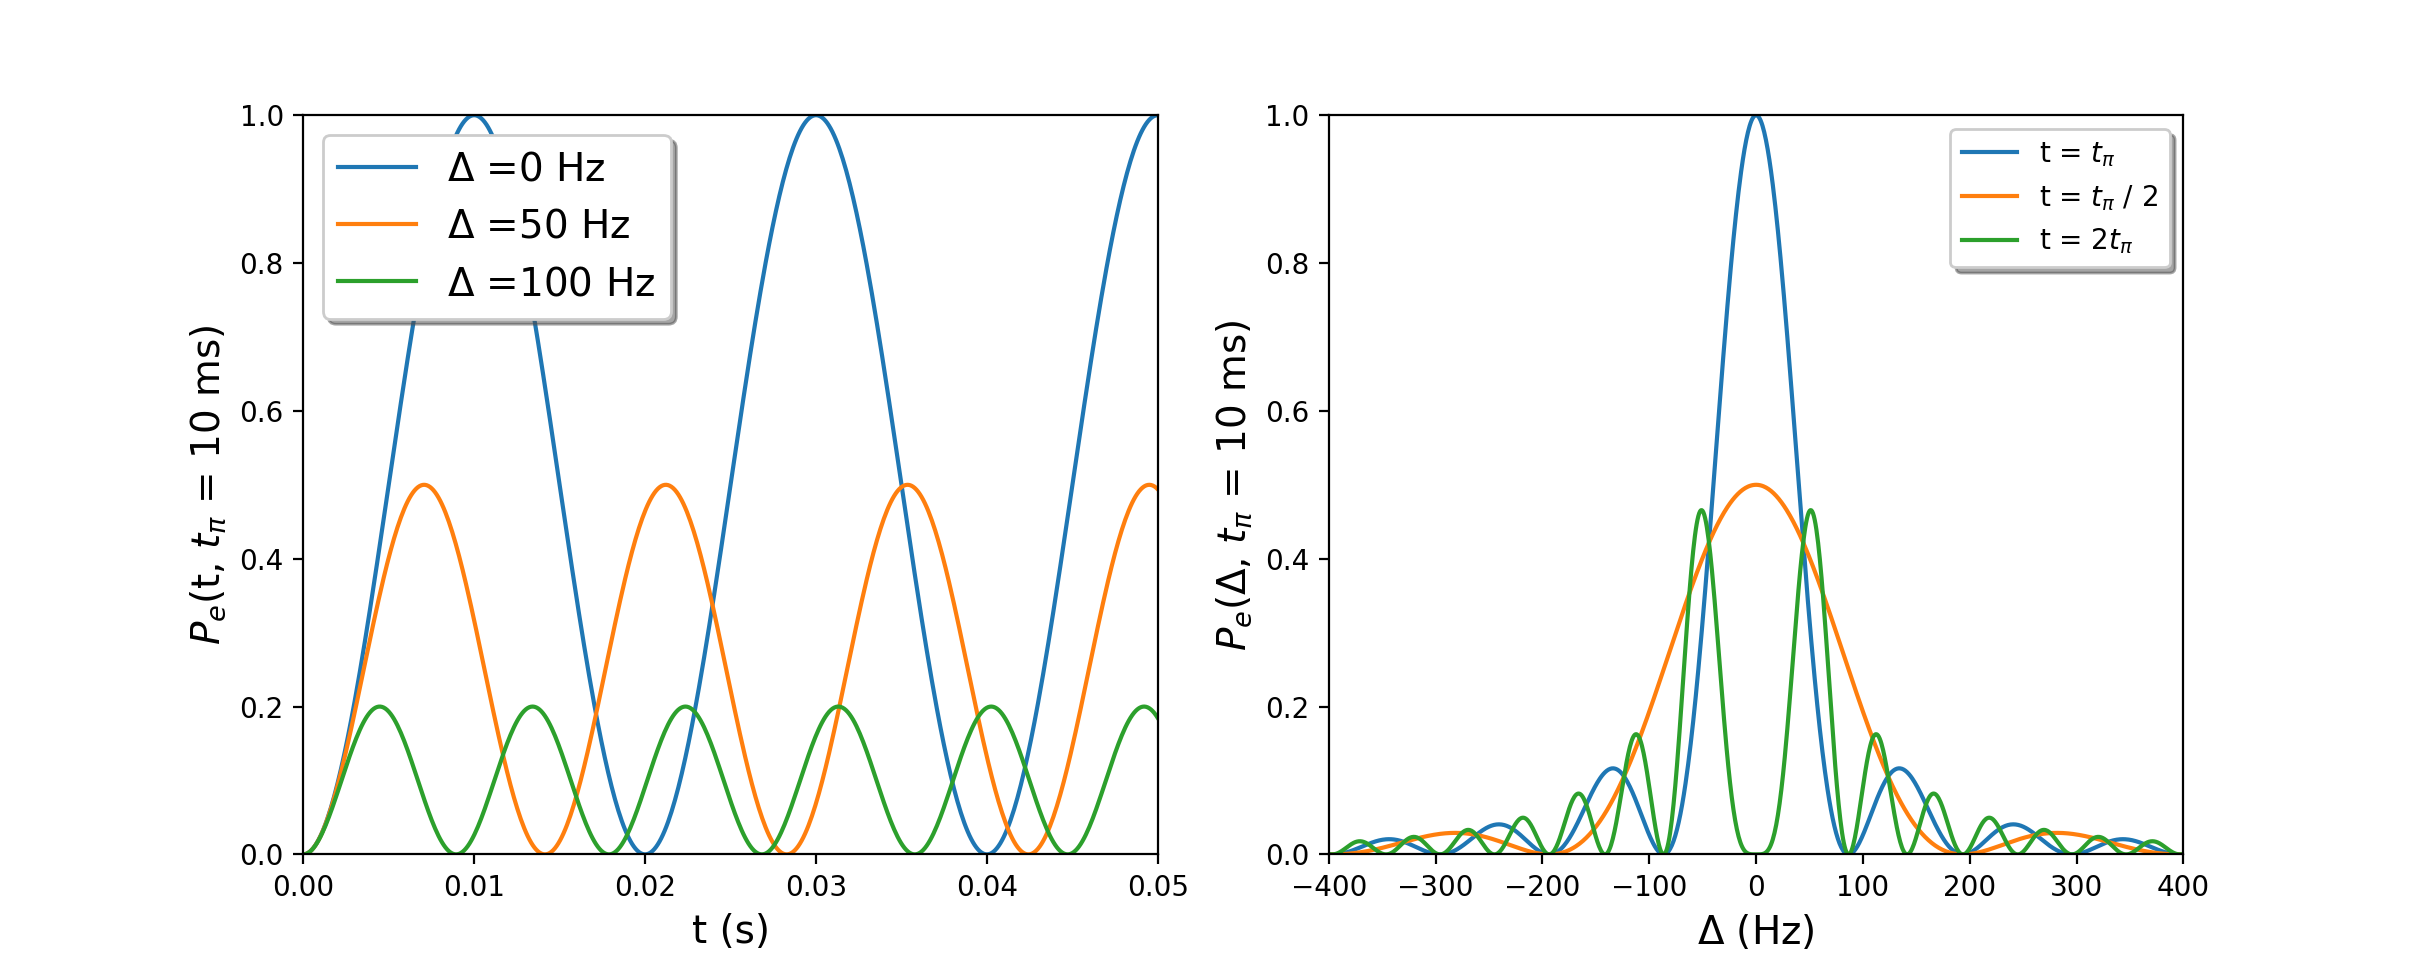
\includegraphics[width=\linewidth]{./plots/Rabi_Oscillations/rabi.png}
\caption{On the right--hand figure it is plotted the transition line shape as a function of the laser detuning from the atomic resonance for different pulse durations. Fixing now the laser frequency with a certain detuning and varying the interaction time or pulse duration, yields to the plot on the left--hand side.}
\label{rabi_osc}
\end{figure}

As you can guess, in the experiment, there are only two parameters that the experimentalist will be interested in to characterize or set up the experiment: $t_{\pi}$ (or the laser intensity) and $\Delta$. It is useful then to re-write the expression for the population of the excited state as a function of these two parameters:

\begin{equation}\label{p_excited}
    P_{e}(t, \Delta) = \left(\frac{\pi}{2}\right)^{2} \left( \frac{ \textrm{sin}\Delta' t/t_{\pi}} {\Delta'} \right)^{2},
\end{equation}

with $\Delta' = \frac{\pi}{2} \sqrt{1 + (t_{\pi} \Delta / \pi)^{2}}  $.

A useful relation is to calculate the Full Width Half Maximum (FWHM) when the laser pulse duration is set to $t_{\pi}$. Defining $P_{e}(t=t_{\pi}, \Delta=\delta/2) = 0.5$ and inserting this in equation \ref{p_excited} we find the equation to solve:
\begin{equation}
    \textrm{sin}\Delta' = \frac{\sqrt{2}\Delta'}{\pi}
\end{equation}
Expanding the sine function we find:
\begin{equation} \label{sinc}
    \begin{cases}
    \sum_{k=0}^{\infty} \frac{(-1)^{k}\Delta'^{2k}}{(2k+1)!} - \frac{\sqrt{2}}{\pi} = 0 \\
    \\
    t_{\pi}\delta = \sqrt{ (\frac{2\Delta'}{\pi})^{2} - 1}
    \end{cases}
\end{equation}

Truncating the series up to $k=3$, we find $t_{\pi}\delta \approx 0.797$, with $\delta$ in Hz. This simple numerical relation tells us that the width of the resonance shape is inversely proportional to the laser pulse duration. Hence, if you are seeking to observe a very narrow atomic resonance using the Rabi spectroscopy scheme (using a $\pi$-pulse to flip the atomic population), the pulse duration may represent a limitation for how narrow the observed transition can be, and in general, this yields in a technical limitation for the precision of experiments.

In the context of optical clocks, where the natural line width of the clock resonances are sub-Hertz, the Rabi profile is the observed resonance shape, limiting the stability of the clocks. The general pratice is then to set $t_{\pi}$ as long as possible. The superior technical limit for the pulse duration is naturally the coherence time of the laser, which, by Fourier transform, is related to the clock laser frequency fluctuations or phase noise. A standard practice is to reference the clock laser to an Ultra Stable Cavity (USC) with a finesse on the order of hundreds of thousands.
The ultimate limit then becames the brownian motion of the cavity mirror coating or thermal agitation, producing a noise in the cavity length and hence noise in the resonance frequency of the cavity which propagates to the laser stabilized to cavity. Solutions to this problem include cryogenic USC and long distance between the mirrors. The coherence time of clock lasers is typically near 1 second.

We quick calculation of the laser line width based on the coherence time of the laser by measuring the longest $t_\pi$ that we can set in the experiment. Let's suppose the ideal case when the laser is turned on at $t=t_{\pi}/2$ and off at $t=t_{\pi}/2$. First step is to calculate the Fourier frequencies associated with this pulse:

\begin{equation}
    \begin{split}
        \mathcal{F}[I(t)] & = \int^{\infty}_{-\infty} I(t) e^{-i\omega t} dt \\
        & = \int^{t_{\pi}/2}_{-t_{\pi}/2} I_{0} e^{-i\omega t} dt \\
        & = I_{0} t_{\pi} \frac{\textrm{sin} (\omega t_{\pi}/2)} {\omega t_{\pi}/2}
    \end{split}
\end{equation}

Now we calculate the width of this profile in the exact same way as in equations \ref{sinc}. This leads to an approximate result:

\begin{equation}
    \Delta \nu _{FWHM} \approx \frac{1.2}{t_{\pi}}
\end{equation}

Hence, for a 1 second coherence time, the laser has an approximate line width of 1.2 Hz, according to this model. From this we conclude that to observe sub-Hertz atomic resonances, laser coherence times longer than 1 s is rquired.

\subsection{Density matrix formalism}


\subsection{Geometrical description: Bloch sphere representation}

A geometrical description a the two-level system can be done by the use of the density operator defined as:
\begin{equation}
    \hat{\rho} = \ket{\psi} \bra{\psi}
\end{equation}
Furthermore, when considering a mixed ensemble, the density operator has to be written as:

\begin{equation}
    \hat{\rho} = \sum_{j} p_{j} \hat{\rho}_{j}, 
\end{equation}

And the statistical average of an observable is calculated as:

\begin{equation} \label{average}
    \langle \hat{A} \rangle = tr(\hat{\rho} \hat{A})
\end{equation}

where the index $j$ refers to a pure state, $p_{j}$ is the probability of this pure state to be found within the ensemble and $\hat{\rho}_{j}$ is the density operator associated to this pure state. For an ensemble of $N$ atoms, $p_{j} = N_{j}/N$. I will first start the discussion regarding a pure state. 

The density operator can be written in a more useful way:
\begin{equation}
    \hat{\rho} = \frac{1}{2} (\mathbb{1} + \vec{r} \cdot \vec{\sigma})
\end{equation}

The vector $\vec{r}$ is called the Bloch vector and $\vec{S} = \vec{\sigma}/2$ is the usual spin $1/2$ operator.
Here is a list of useful relations concerning the $\sigma$ operators:

\begin{equation}
\begin{cases}
    [\sigma_{i}, \sigma_i]  = 2 i \varepsilon_{ijk} \sigma_{k} \\
    \sigma_{i}^{2} = \mathbb{1} \\
    \sigma_{i} \sigma_{j} \sim \sigma_{k} \\
    tr(\sigma_{i}) = 0
\end{cases}
\end{equation}

Now, using the expression \ref{average}, we can show that:

\begin{equation}
    \langle \sigma_{i} \rangle = r_{i}
\end{equation}

This expression tells us that the components of the Bloch vector are just the averages of the Pauli operators
$\langle \sigma_{i} \rangle = \bra{\psi} \sigma_{i} \ket{\psi}$. In terms of the elements of the density matrix:

\begin{equation}
\begin{cases}
    r_{x} = 2 \mathrm{Re}(\rho_{01})\\
    r_{y} = 2 \mathrm{Im}(\rho_{10}) \\
    r_{z} = \rho_{00} - \rho_{11}
\end{cases}
\end{equation}

The Bloch vector, as defined above, has three real numbers that completely specify the probability amplitudes in the wavefunction. For a pure state the Bloch vector is a unit vector and all possible vectors lie on a sphere of radius 1. For mixed states the Bloch vector lies within the sphere.
Writting the wavefunction as $\ket{\psi} = \phi_{0} \ket{0} + \phi_{1} \ket{1}$:

\begin{equation}
\begin{cases}
    \rho_{00} = |\phi_{0}|^{2} \\
    \rho_{11} = |\phi_{1}|^{2} \\
    \rho_{01} = \phi_{0}\phi_{1}^{*} \\
    \rho_{10} = \rho_{01}^{*}
\end{cases}
\end{equation}

In this view, is it interesting to note that a rotation applied to the wavefunction leads to exact same rotation of the Bloch vector. Let's consider the rotation operator $\hat{D}(R)$:

\begin{equation}
    \hat{D}(R) \ket{\psi} = \ket{\psi}_{r}
\end{equation}

And the rotation on operators:

\begin{equation}
    \hat{D}(R) \hat{O} \hat{D}(R)^{-1} = \hat{O}_{r}
\end{equation}

Applying the rotation to the density operator:

\begin{equation}
    \hat{D}(R) \hat{\rho} = \frac{1}{2}(\mathbb{1} + \vec{r}\cdot \hat{D}(R) \vec{\sigma} \hat{D}(R)^{-1})
\end{equation}

Which is equivalent to calculate the density operator in terms of the rotated states:

\begin{equation}
    \hat{\rho}_{r} = \ket{\psi}_{r} \bra{\psi}_{r}
\end{equation}

Here the name rotation wave approximation makes more sense. The unitary time evolution operator $e^{-i \omega_{L} t \sigma_{z}/2}$ is a rotation of the Bloch vector around the z component with angular frequency $\omega_{L}$.
The unitary transformation consists in applying the reverse time evolution operator in order to cancel this rotation. Or, a transformation to a counter-rotating frame. Indeed, in the basis {$\ket{0}, \ket{1}$}:

\[
e^{- i \omega_{L}t \hat{\sigma}_{z}/2} =
  \begin{bmatrix}
    e^{- i \omega_{L}t/2} & 0  \\
    0 & e^{ i \omega_{L}t /2}
  \end{bmatrix}
\]

Now, looking at the Hamiltonian \ref{h_int}, we can tell now that the effect of the laser interaction on resonance is to rotate the Bloch vector around the x axis with angular frequency $2\Omega_{R}$. If not on resonance, rotations around the z axis are expected. Another way to see this is to understand that the detuning changes the rotation axis. Re-writting the Hamiltonian \ref{h_int} in the general rotation rotation operator form:

\begin{equation} \label{h_n}
    \mathcal{H} = \frac{\hbar \Omega'}{2} \vec{\sigma}_{n}
\end{equation}

With, $\vec{\sigma}_{n} = \frac{\vec{n}}{|\vec{n}|} \cdot \vec{\sigma}$ and:

\begin{equation}
    \hat{n} = \frac{- \Delta \hat{z} + 2\Omega_{R} \hat{x}} {\Omega'}
\end{equation}

THe Hamiltonian \ref{h_n} has now a simple and beautiful interpretation: a rotation of the Bloch vector around the axis defined by the vector $\vec{n}$ with angular frequency $\Omega'$.

The initial condition $p_{0}(0) = 1$ is represented by a Bloch vector pointing up in the z axis, and after a $\pi$ pulse on resonance the vector rotates around the x-axis and ends at the z axis pointing down and the population is inverted: $p_{1}(t_{\pi}) = 1$. A $\pi /2$ pulse leaves the Bloch vector on the y axis and the wavefunction is:

\begin{equation}
    \ket{\psi (t = \pi/2)} = \frac{1}{\sqrt{2}}(\ket{0} - i \ket{1})
\end{equation}

In general, quantum state manipulations with laser interaction is represented by unitary time evolution operators which represent rotations of the Bloch vector around a given axis by an angle $\theta = \Omega t$:

\begin{equation}
    \ket{\psi}_{r} = \mathcal{U} \ket{\psi}
\end{equation}

\begin{equation}
    \mathcal{U} = e^{- i \Omega t \hat{\sigma}_{\vec{n}} /2}
\end{equation}

\section{Ensemble of two-level atoms: mixed states}

\end{document}